\documentclass[a4paper]{article}

\usepackage[a4paper,top=2cm,bottom=2cm,left=3cm,right=3cm,marginparwidth=1.75cm]{geometry}
\usepackage[utf8]{inputenc}
\usepackage[T1]{fontenc}
\usepackage{textcomp}
\usepackage[ngerman]{babel}
\usepackage{amsmath, amssymb, nccmath}
\usepackage{accents}


\usepackage{multirow}
\usepackage{fancyhdr}
\usepackage{lastpage}

% figure support
\usepackage{import}
\usepackage{xifthen}
\pdfminorversion=7
\usepackage{pdfpages}
\usepackage{transparent}
\newcommand{\incfig}[1]{%
    \def\svgwidth{\columnwidth}
    \import{./figures/}{#1.pdf_tex}
}

\pdfsuppresswarningpagegroup=1

\title{Protokoll zur ersten Laborübung\\Messtechnik Labor 376.091}
\author{DINC Atilla (11917652)}

\begin{document}
\newcommand{\unit}[1]{\ensuremath{\, \mathrm{#1}}} % Einheiten in Math-Moder richtig formatieren
% --------------------- HEADER ---------------------
\pagestyle{fancy}
% --------------------- FOOTER ---------------------
\fancyfoot[L]{Wintersemester 2023}
\fancyfoot[C]{\textbf{\thepage /\pageref{LastPage}}}
\renewcommand{\footrulewidth}{0.4pt}

\normalsize
\maketitle
\tableofcontents

\begin{center}
	\begin{tabular}{|c| c| c| c| c|}
		\hline
		\multicolumn{5}{|c|}{\textbf{Geräteliste}}                                                                                        \\
		\hline

		Bezeichnung              & Gerätebeschreibung                                         & Messgrößen & Inventarnummer & Bemerkungen \\
		\hline
		MM0                      & Agilent Digitalmultimeter True RMS                                  & -          & U1232A         & -           \\
		MM1                      & Digitalmultimeter                                          & -          & \#11            & -           \\
		MM2                      & Digitalmultimeter                                          & -          & \#7             & -           \\
		%\multirow{2}{*}{OZ1}     &
		%\multirow{2}{*}{
		%\begin{tabular}[c]
		%		Digitalspeicheroszilloskop DSO-x2002A \\
		%		MMSR
		%	\end{tabular}
		%}& \multirow{2}{*}{-} & \multirow{2}{*}{C0404-5} & \multirow{2}{*}{-}  \\
		                         &                                                            &            &                &             \\
		NG1                      & Netzgerät 2-Channel $\pm10\unit{mV}$                       & -   & CD0404-6       & -           \\
		FG1                      & Funktionsgenerator                                         & -    & SDG1025        & -           \\
		\hline
		\hline
		\multicolumn{5}{|c|}{\textbf{Zubehörliste}}                                                                                       \\
		\hline

		Bezeichnung              & Zubehörbeschreibung                                        & Messgrößen & Inventarnummer & Bemerkungen \\
		\hline
		K1                       & Tastkopf (10:1) 100\unit{MHz} 10\unit{M\Omega} 15\unit{pf} & -          & -              & grau         \\
		K2                       & Tastkopf (10:1) 150\unit{MHz} 10\unit{M\Omega} 15\unit{pf} & -          & -              & rot       \\
		K3                       & Tastkopf (10:1) 150\unit{MHz} 10\unit{M\Omega} 15\unit{pf} & -          & -              & rosa        \\
		\hline
	\end{tabular}
\end{center}
\newpage
% ~~~~~~~~~~~~~~~~~~~~~~~~~~~~ Start of the document ~~~~~~~~~~~~~~~~~~~~~~~~~~~~

\section{Einleitung}

\section{Messungen mit dem Digitalmultimeter}
\subsection{Spannungsmessung}
Zur Spannungsmessung wird der Spannungseingang des Multimeters parallel zur Messgröße
geschaltet, daher ist ein möglichst hoher Innenwiderstand $R_{i}$ erwünscht. Zur
Bestimmung dieses Innenwiderstands $R_{i}$ sollte eine Serienschaltung mit einem 
relativ hochohmigen bekannten Widerstand aufgebaut und der Spannungsabfall am Multimeter
von diesem abgelesen werden.\newline
Weiters sollte der Einfluss des Multimeters auf die Schaltung gemessen werden,
indem der Spannungseingang eines Multimeters des gleichen Models parallel zum 
Multimeter angeschlossen wird. \newline
Zuletzt sollte eine Messbereichserweiterung durchgeführt werden, indem ein
Serienwiderstand bekannter Größe in den Strompfad verbaut und der 
Spannungsabfall gemessen wird gemessen wird.

\subsubsection{Messaufbau und Messdurchführung}
\subsubsection*{Bestimmung des Innenwiderstands}
Die eingestellte Spannung des Netzgerätes FG1 wurde mit dem Multimeter MM0 
geprüft bevor sie mit der Schaltung belastet wurde. Der Serienwiderstand R1 wurde
mit dem Multimeter MM0 bestimmt.
Im Anschluss wurde die Schaltung wie in Abb. \ref{fig:1a_RiVM} angeschlossen.
Die angezeigte Spannung am Multimeter MM1 wurde abgelesen und die Eingangsspannung
wurde erneut gemessen. Weder die Eingangsspannung, noch die Spannung am Multimeter
MM1 haben sich geändert. Somit wurde sichergestellt, dass sowohl Innenwiderstand
des Netzgerätes, als auch jegliche Kontaktwiderstände in der Schaltung
vernachlässigbar klein für unsere Messungen waren.\newline
Der Kontrollprozess wurde vor allen folgenden Messungen durchgeführt, um die
Eingangsspannung möglichst genau zu bestimmen.
\begin{figure}[h]
    \centering
    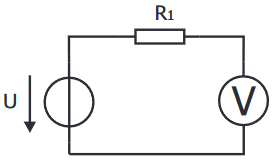
\includegraphics[width=0.4\textwidth]{schematics/1a_RiVM.png}
    \caption{Schaltung zur Bestimmung des Multimeter-Innenwiderstands}
    \label{fig:1a_RiVM}
\end{figure}

\subsubsection*{Bestimmung des Einflusses}
Für diese Messung wurde die Eingangsspannung $U_{q}$ wie zuvor gemessen.
Als Widerstand $R_{M}$ wurde der gleiche Widerstand wie zuvor verwendet und auch
und auch das Multimeter MM1 wurde nicht gewechselt, somit konnte die vorherige
Schaltung beibehalten und wie in Abbildung \ref{fig:1b_EinflussVM} erweitert werden.
Die Spannungen an den Multimetern wurden zunächst mit nur einem Multimeter MM1
und danach mit beiden Multimetern MM1 und MM2 abgelesen.
\begin{figure}[h]
    \centering
    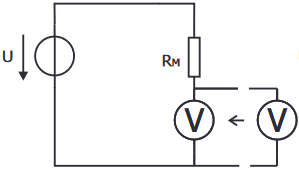
\includegraphics[width=0.4\textwidth]{schematics/1b_EinflussVM.png}
    \caption{Schaltung zur Bestimmung des Einflusses}
    \label{fig:1b_EinflussVM}
\end{figure}

\subsubsection*{Messbereichserweiterung}
Zur Messbereichserweiterung wurde die Schaltung wie in Abb. \ref{fig:1c_MB-ErweiterungVM}
aufgebaut. Dabei wurde der Widerstand $R_{M}$ aus der vorherigen Schaltung
und zur Messbereichserweiterung verwendet. Die zu messenden Spannungen in dieser
Schaltung ist die Eingangsspannung $U_{q}$ und sie soll in etwa halbiert werden, indem
die Widerstände mit $R_{M}\approx R_{V}$ auch in etwa gleich groß gewählt werden.
\begin{figure}[h]
    \centering
    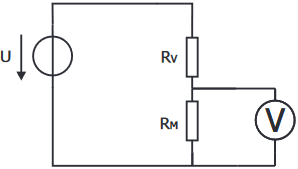
\includegraphics[width=0.4\textwidth]{schematics/1c_MessbereichserweiterungVM.png}
    \caption{Schaltung zur Messbereichserweiterung eines Voltmeters}
    \label{fig:1c_MB-ErweiterungVM}
\end{figure}

\subsubsection{Messergebnisse}
\subsubsection*{\textbf{Bestimmung des Innenwiderstands}}
Die Schaltung wurde mit einer gemessenen Eingangsspannung $U_{q}=9,92\unit{V}$ und einem
gemessenen Widerstand $R_{1}=98,9 \unit{k\Omega}$ aufgebaut. Weiters wurde am
Multimeter MM2 die Spannung $U_{V}=9,84\unit{V}$ gemessen. Mithilfe der Formel
für den Spannungsteiler kann die Gleichung
\[ U_{V}=U_{q} \frac{R_{i}}{R_{1}+R_{i}} = U_{q} \frac{1}{1 + \frac{R_{1}}{R_{i}}}\]
aufgestellt werden, woraus sich direkt durch Umformung
\[ R_{i}=\frac{R_{1}}{\frac{U_{q}}{U_{v}}-1}\approx 12,1647 \unit{M\Omega} \]
ergibt.

\subsubsection*{\textbf{Bestimmung des Einflusses}}
Auch bei dieser Messung wurde mit dem Handmultimeter MM0 eine Eingangsspannung
$U_{q}=9,92V$ verifiziert. Der Widerstand wurde wieder zu $R_{1}=98,9 \unit{k\Omega}$ gemessen.
Damit wurden die Messergebnisse wie in Tabelle \ref{tab:1b_Ergebnisse} aufgenommen.
Der Einfluss ergibt sich zur relativen Abweichung
\[ \Delta u_\text{MM1[\%]} =
        \frac{9,73\unit{V} - 9,84\unit{V}}{9,84\unit{V}} \cdot 100
    \approx -1,12\% .\]
\begin{table}[h]
    \centering
    \caption{Messergebnisse zum Einfluss eines Voltmeters}
    \label{tab:1b_Ergebnisse}
    \begin{tabular}{|c|c|c|}
        \hline
         & $U_{\text{MM1}}$&  $U_{\text{MM2}}$\\ 
        \hline
        vorher &$9,84\unit{V}$& $-$\\
        \hline
        nachher &$9,73\unit{V}$& $9,71\unit{V}$\\
        \hline
    \end{tabular}
\end{table}

\subsubsection*{Messbereichserweiterung}
Auch hier wurden die Eingangsspannung $U_{q}=9,92\unit{V}$ sowie der Widerstand 
$R_{M}=98,9\unit{k\Omega}$ gemessen. Weiters wurde der Widerstand
$R_{V}=99,5\unit{k\Omega}$ gemessen. Mit dem gemessenen Spannungsabfall
$U_{M}=4,93\unit{V}$ kann die Eingangsspannung $U_{q}$ über das messbereichserweiterte
Multimeter gemessen werden.
Aus der Maschengleichung folgt direkt
\[ U_{q}=R_{V}I+U_{M} = R_{V} \bigg(\frac{U_{M}}{R_{M}} + \frac{U_{M}}{R_{i}}\bigg) + U_{M} \]
\[ \implies U_{q}=U_{M}\bigg(1+\frac{R_{V}}{R_{M}} + \frac{R_{V}}{R_{i}} \bigg)
\approx 9,93 \unit{V}\]
\[ \implies f_{ME}=\frac{U_{q}}{U_{M}}\approx  2,0142\]


\subsection{Strommessung}
Ähnlich zur Messung mit einem Voltmeter wird auch bei einer Strommessung die
Schaltung durch das Amperemeter belastet. Da ein Amperemeter seriell zum
stromdurchflossenen Bauteil verschaltet wird, muss der Innenwiderstand möglichst
klein sein, um einen möglichst keinen Spannungsabfall zu verursachen.
Weiters kann der Messbereich eines Amperemeters erweitert werden, indem der
"überschüssige" Strom über einen parallelen Widerstand abgeführt wird.\newline
In diesem Abschnitt sollten analoge Schritte wie bei der Spannungsmessung durchgeführt werden: 
der Innenwiderstand $R_{i}$ und der Einfluss auf die Schaltung sollen bestimmt 
und eine Messbereichserweiterung sollte durchgeführt werden.

\subsubsection{Messaufbau und Messdurchführung}
\subsubsection*{Bestimmung des Innenwiderstands}

\begin{figure}[h]
    \centering
    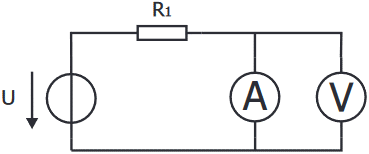
\includegraphics[width=0.4\textwidth]{schematics/2a_RiAM.png}
    \caption{Schaltung zur Bestimmung des Innenwiderstands}
    \label{fig:2a_RiAM}
\end{figure}

\subsubsection*{Bestimmung des Einflusses}

\begin{figure}[h]
    \centering
    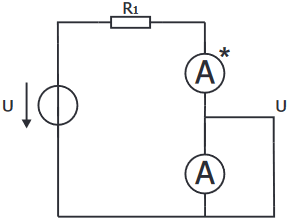
\includegraphics[width=0.4\textwidth]{schematics/2b_EinflussAM.png}
    \caption{Schaltung zur Bestimmung des Einflusses}
    \label{fig:2b_EinflussAM}
\end{figure}

\subsubsection*{Messbereichserweiterung}

\begin{figure}[h]
    \centering
    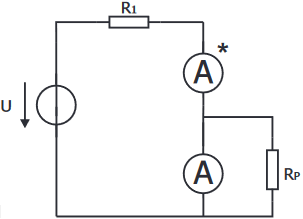
\includegraphics[width=0.4\textwidth]{schematics/2c_MessbereichserweiterungAM.png}
    \caption{Schaltung zur Messbereichserweiterung}
    \label{fig:2c_MB-ErweiterungAM}
\end{figure}

\subsubsection{Messergebnisse}
\subsubsection*{Bestimmung des Innenwiderstands}
Die tatsächliche Größe des Vorwiderstands wurde mit dem Handmultimeter vermessen
und betrug $R_{1}=4,68\unit{k\Omega}$.
Nachdem ein Anzeigestrom am Amperemeter von $I_{A}=500\unit{µA}$ eingestellt wurde,
stellten sich eine Gesamtspannung $U_{q}=2,382\unit{mV}$ und eine Spannung am
Amperemeter $U_{A}=50,5 \unit{mV}$ ein.\newline
Es lässt sich direkt der Innenwiderstand berechnen zu
\[ R_{i}= \frac{U_{A}}{I_{A}}= 101\unit{\Omega} ,\]
dieses Ergebnis ist für den niedrigen Strombereich des Multimeters sinnvoll.

\subsubsection*{Bestimmung des Einflusses}
Wie auch zuvor wurden Vorwiderstand $R_{1}=4,68\unit{V}$ sowie
Gesamtspannung $U_{q}=2,413V$ vermessen. Nach der Messung wurden die
Messergebnisse aus Tabelle \ref{tab:2b_EinflussAM} aufgenommen.
\[ f_{A}=\frac{490\unit{\mu A}}{500\unit{\mu A}} =0,98\]
\begin{table}[h]
    \centering
    \caption{Messergebnisse zum Einfluss des Amperemeters}
    \label{tab:2b_EinflussAM}
    \begin{tabular}{|c|c|c|}
        \hline
     & $I_{A}$  & $I_{A*}$\\ 
     \hline
        vorher & - & $500\unit{\mu A}$ \\
        \hline
        nachher & $495\unit{\mu A}$ & $490\unit{\mu A}$\\
     \hline
    \end{tabular}
\end{table}

\subsubsection*{Messbereichserweiterung}
Der gemessene Parallelwiderstand betrug $R_{P}=9,9\unit{k\Omega}$.
Mit diesem Widerstand wurde die Zweigströme $I_{A*}=500\unit{\mu A}$ und
$I_{A}=499\unit{\mu A}$ gemessen.
\[ \implies f_{ME}=\frac{I_{A*}}{I_{A}}\approx 1,002 \]
Diese Werte haben sich bei einer Versorgungsspannung $U_{q}=2,458\unit{V}$ eingestellt.

\subsection{Widerstandsmessung}
Hier sollten ein $100\unit{\Omega}$ und ein $100 \unit{k\Omega}$ Widerstand vermessen werden.
Dazu muss direkt mit einem Ohmmeter und über den Strom und die Spannung gemessen
werden. Weiters muss der Farbcode identifiziert werden.

\subsubsection{Messaufbau und Messdurchführung}
\subsubsection*{\textbf{Widerstandsfarbcode}}
Die Widerstände $R_{1,G}$ und $R_{1,K}$ wurden zunächst über ihren Farbcode identifiziert und ausgewählt.

\subsubsection*{Direkte Messung}
Mit dem Digitalmultimeter MM0 wurden sowohl $R_{1,G}$ als auch $R_{1,K}$ vermessen.
Dadurch konnte schonmal sichergestellt werden, dass die Widerstandsfarbcodes richtig
gelesen wurden.

\subsubsection*{Strom- und Spannungsmessung}
Zur Bestimmung des Widerstandes über den Zusammenhang des ohmschen Gesetztes musste
bedacht werden, dass es zwei unterschiedliche Messmethoden gibt:
\begin{itemize}
    \item Stromrichtige Messung:
        Vorallem bei sehr großen Widerständen gut geeignet. Hierfür wurde das
        Multimeter MM1 als Amperemeter und das Multimeter MM2 als Voltmeter verwendet.
        \begin{figure}[h]
            \centering
            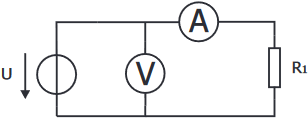
\includegraphics[width=0.4\textwidth]{schematics/3a_stromrichtigeWidMessung.png}
            \caption{Schaltung zur stromrichtigen Widerstandsmessung}
            \label{fig:3a_stromrichtigeWidMessung}
        \end{figure}
    \item Spannungsrichtige Messung:
        Vorallem bei sehr kleinen Widerständen gut geeignet. Hierfür wurde das
        Multimeter MM1 als Amperemeter und das Multimeter MM2 als Voltmeter verwendet.
        \begin{figure}[h]
            \centering
            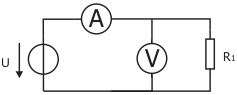
\includegraphics[width=0.4\textwidth]{schematics/3b_spannungsrichtigeWidMessung.png}
            \caption{Schaltung zur spannungsrichtigen Widerstandsmessung}
            \label{fig:3b_spgsrichtigeWidMessung}
        \end{figure}
\end{itemize}
Für diese Laborübung sollen beide Methoden an beiden Widerständen durchgeführt werden.
Zur Durchführung wurde eine Versorgungsspannung gewählt, die für beide Widerstände
geeignet ist und möglichst groß ist. Dadurch wird die Messgenauigkeit der
Messgeräte möglichst gut ausgenutzt.
Zur Durchführung wurde eine Versorgungsspannung gewählt, die für beide Widerstände
geeignet ist und möglichst groß ist. Dadurch wird die Messgenauigkeit der
Messgeräte möglichst gut ausgenutzt. Mit einer Eingangsspannung $U_{q}\approx 2V$
liegen beide Widerstände weit von ihrer thermischen Belastungsgrenze entfernt.

\subsubsection{Messergebnisse}
\subsubsection*{Widerstandsfarbcode}
Das Auslesen des Widerstandsfarbcodes hat die Widerstände
\begin{itemize}
    \item $R_{1,K}=(100 \pm 5\% )\unit{\Omega}$
    \item $R_{1,G}=(100 + \pm 5 \%)\unit{k\Omega}$
\end{itemize}
ergeben.

\subsubsection*{Direkte Messung}
Die direkte Messung mit einem Multimeter hat die Widerstände
\begin{itemize}
    \item $R_{1,K}=98,5\unit{\Omega}$
    \item $R_{1,G}=99,7\unit{k\Omega}$
\end{itemize}
ergeben.

\subsubsection*{Stromrichtige Messung}
Als Versorgungsspannung wurde $U_{q}=1,989\unit{V}$ gewählt. Daraus ergaben sich die Messungen
\begin{itemize}
    \item niederohmiger Widerstand: $U_{K}=1,97\unit{V}$, $I_{K}=19,6\unit{mA}$
        $\implies R_{1,K}= \frac{U_{K}}{I_{K}}\approx 100,51\unit{\Omega}$
    \item hochohmiger Widerstand: $U_{G}=1,97\unit{V}$, $I_{G}=20,0\unit{\mu A}$
        $\implies R_{1,K}= \frac{U_{K}}{I_{K}}\approx 98,5\unit{k\Omega}$
\end{itemize}
ergeben.\newline


\subsubsection*{Spannungsrichtige Messung}
Als Versorgungsspannung wurde $U_{q}=1,989\unit{V}$ gewählt. Daraus ergaben sich die Messungen
\begin{itemize}
    \item niederohmiger Widerstand: $U_{K}=1,85\unit{V}$, $I_{K}=19,04\unit{mA}$
        $\implies R_{1,K}= \frac{U_{K}}{I_{K}}\approx 97,164\unit{\Omega}$
    \item hochohmiger Widerstand: $U_{G}=1,976\unit{V}$, $I_{G}=18,4\unit{\mu A}$
        $\implies R_{1,K}= \frac{U_{K}}{I_{K}}\approx 107,39\unit{k\Omega}$
\end{itemize}
ergeben.

\subsubsection*{Fazit}
Wie erwartet war die stromrichtige Messung viel genauer bei der Messung des
hochohmigen Widerstands und die spannungsrichtige Messung war besser für die
Messung des niederohmigen Widerstands geeignet. Die Direkte Messung war in
beiden Fällen sehr akkurat und die Bestimmung über den Farbcode ging am
schnellsten, sofern man die Kodierung schnell entschlüsseln konnte.

\newpage
\section{Messungen mit dem Oszilloskop}
Mithilfe des Oszilloskops können alle signalform-abhängigen Eigenschaften
untersucht werden, weshalb sich dieses für detailierte Untersuchungen besonders
gut eignet, aber auch eine aufwändigere Messung fordert. Nicht nur die
Interpretation der Ergebnisse ist komplexer, auch die Kenntnisse über das
Messgerät und vom Zubehör müssen besser sein.

\subsection{Tastkopf}
Tastköpfe mit einem einstellbaren Tastverhältnis werden oft mit einer verstellbaren
Kapazität ausgestattet. Durch Veränderung der Kapazität kann der interne
komplexe Spannungsteiler kompensiert werden. In dieser Übung sollen drei Tastköpfe
K1, K2 und K3 mithilfe des Oszilloskops OZ1 kompensiert werden. Dabei soll ein
Tastkopf möglichst gut kompensiert werden, einer soll überkompensiert und der dritte
soll unterkompensiert werden. Dabei soll ein
Tastkopf möglichst gut kompensiert werden, einer soll überkompensiert und der dritte
soll unterkompensiert werden.

\subsubsection{Messaufbau und Messdurchführung}
Es wurden drei kompensierbare Tastköpfe mit unterschiedlichen Markierungen herausgesucht.
Diese wurden nacheinander am Channel 1 Eingang des Oszilloskops OZ1 angeschlossen
und am Rechteck-Ausgang des Oszilloskops kompensiert. 
\begin{itemize}
    \item Tastkopf K1 wurde dem Rechtecksignal möglichst gut angenähert und 
        somit \textbf{abgeglichen}.
    \item Tastkopf K2 wurde \textbf{unterkompensiert}, sodass die Flanken möglichst
        abgerundet waren.
    \item Tastkopf K3 wurde \textbf{überkompensiert}, sodass starke Überschwingungen an
        den Flanken auftraten.
\end{itemize}
Zur Messung wurde als nächstes ein Sinussignal ($f=[100, 100\unit{k}]\unit{Hz}$,
$10\unit{V_{pp}}$) über ein passendes Endstück aus dem Funktionsgenerator FG1
ausgeführt und dessen Spitze-Spitze-Spannung vermessen. Schließlich wurden die
Signalverläufe der Tastköpfe K1 und K3 verglichen und deren Phasenverschiebung vermessen.
\subsubsection{Messergebnisse}
Die Messung der Spitzenwerte sind in Tabelle \ref{tab:4a_Vpp} ersichtlich und
und wurden mit der Measure-Funktion des Oszilloskops gemessen. Während der
abgeglichene Tastkopf den Messdaten nach komplett Frequenzunabhängig ist, weist
der überkompensierte Tastkopf K3 extreme Spannungserhöhungen mit steigender
Frequenz und der unterkomensierte Tastkopf K2 extreme Spannungsabschwächungen
mit steigender Frequenz auf.\newline
In Abb. \ref{fig:4b_VergleichK1K2} ist zusätzlich zum Unterschied in der Ampltiude
eine Phasenverschiebung zu erwarten. Durch manuelle Messung mittels der
Cursor-Funktion des Oszilloskops ergibt sich eine vernachlässigbare Phasenverschiebung
\[ \Delta \phi=\frac{\Delta T}{T}2\pi=\frac{1,34 \unit{\mu s}}{100 \unit{\mu s}}2\pi¸\approx 0,084^\circ .\]


\begin{table}[h]
    \centering
    \caption{Spitze-Spitze-Spannungen gemessen mit unterschiedlich kompensierten Tastköpfen}
    \label{tab:4a_Vpp}
    \begin{tabular}{|c|c|c|c|}
        \hline
        $f$ in $\unit{kHz}$& K1 in $V_{pp}$ & K2 in $V_{pp}$& K3 in $V_{pp}$\\ 
     \hline
        $0,1$ & $10,6$ & $10,5$& $10,7$ \\
        $1  $ & $10,6$ & $10,09$& $12,3$  \\
        $10 $ & $10,6$ & $5,41$& $17,9$ \\
        $100$ & $10,6$ & $5,04$& $18,3$ \\
        \hline
    \end{tabular}
\end{table}
\begin{figure}[h]
    \centering
    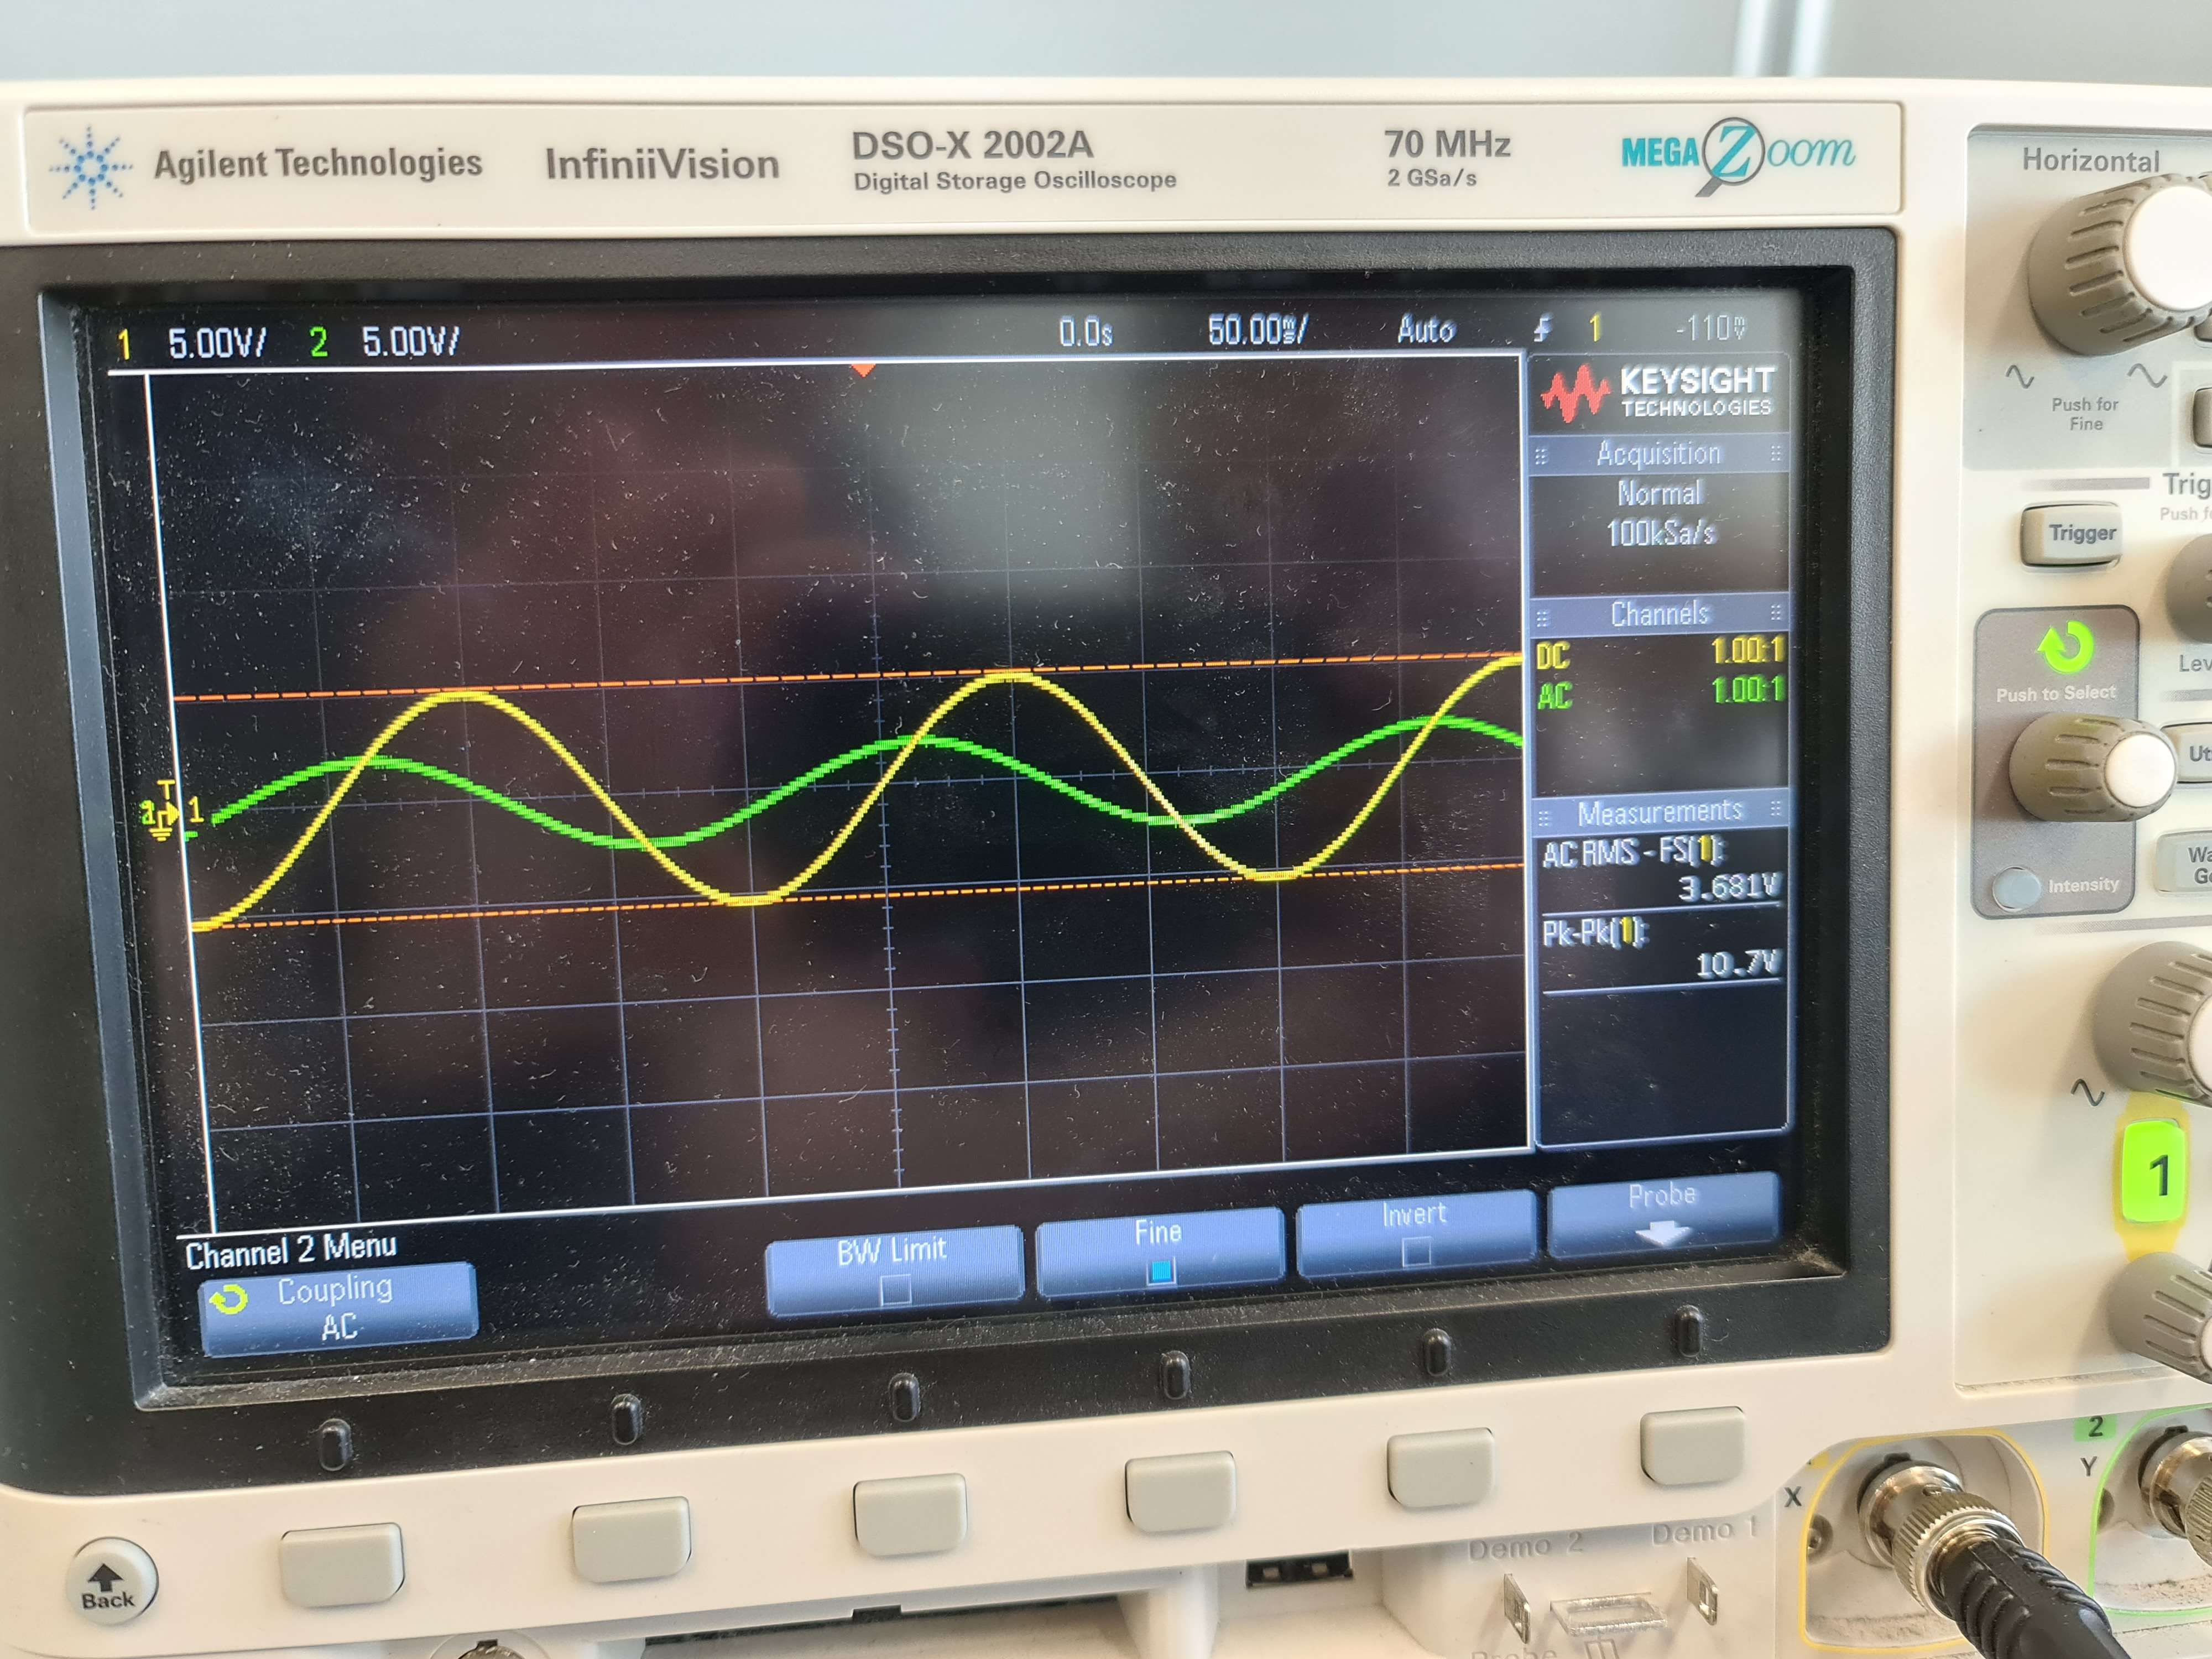
\includegraphics[width=0.8\textwidth]{images/Oszi - Sinus.jpg}
    \caption{Vergleich Tastkopf 1 (Sinus mit kleinerer Amplitude) und Tastkopf 2 (Sinus mit größerer Amplitude)}
    \label{fig:4b_VergleichK1K2}
\end{figure}

\subsection{AC-Spannungsmessung}
Hier sollten unterschiedliche, periodische Signalformen miteinander Verglichen werden.
Dazu müssen die Kenngrößen Spitzenwert und Effektivwert herangezogen werden.

\subsubsection{Messaufbau und Messdurchführung}
Zunächst wurde die Schaltung wie in Abb. \ref{fig:5a_ACMessung} mit den 
Widerständen $R_{1}=100\unit{\Omega}$, $R_{2}=4,7\unit{k\Omega}$ und
$R_{3}=100\unit{k\Omega}$ aufgebaut und der Funktionsgenerator auf mit $U_{pp}=1\unit{V_{pp}}$ eingestellt.
Um die Spannung zur gemeinsamen Masse zwischen Oszilloskop OZ1 und Funktionsgenerator FG1
und Oszilloskop abgreifen zu können, wurde der Widerstand $R_{2}$ dritter Stelle,
an der Masse angebracht. Am Funktionsgenerator wurde der der $50\unit{\Omega}$
Ausgang eingestellt. Das Signal wurde über ein Koax-Kabel mit dem Oszilloskop verbunden
und das Tastverhältnis $1:1$ richtig eingestellt.\newline
Mit dem Oszilloskop wurden die Kennwerte für Sinus-, Dreieck- und Rechteckformen gemessen. Der Ausgang des
Funktionsgenerators wurde auf HIGH-Z gestellt und die Messungen wurden wiederholt.
\begin{figure}[h]
    \centering
    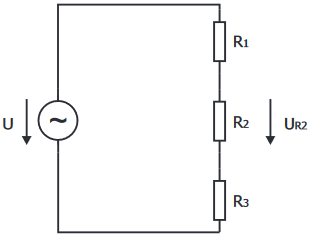
\includegraphics[width=0.4\textwidth]{schematics/5a_ACMessung}
    \caption{Schaltung zur AC-Spannungsmessung}
    \label{fig:5a_ACMessung}
\end{figure}

\begin{table}[h]
    \centering
    \caption{Messung der Kennwerte unterschiedlicher Signalformen}
    \label{tab:5b_Kennwerte}
    \begin{tabular}{|c|c|c|c|c|c|}
        \hline
        $f\unit{[kHz]}$ & Signalform & $U_{pp,HighZ}\unit{[mV_{pp}]}$ & $U_{pp,50\Omega}\unit{[mV_{pp}]}$ &
        $U_{RMS,HighZ}\unit{[mV_{RMS}]}$ & $U_{RMS,50\Omega}\unit{[mV_{RMS}]}$\\
        \hline
        $1$& Sinus & $950$ & $950$ & $331$ & $331$\\
        $1$ & Dreieck & $941$ & $943$ & $270$ & $270$ \\
        $10$ & Dreieck & $950$ & $946$ & $272$ &  $270$\\
        $100$ & Dreieck & $960$ & $960$ & $273$ & $273$\\
        $1$ & Rechteck & $942,75$ & $937,25$ & $474$ & $470$\\
        $10$ & Rechteck & $950$ & $950,5$ & $474$ & $473$\\
        $100$ & Rechteck &  $956$ & $943$ & $477$ & $476$\\
        \hline
    \end{tabular}
\end{table}

\subsection{RMS im Detail}
Mit einem ähnlichen Aufbau wie bei der AC-Messung soll nun die RMS-Funktionalität
unterschiedlicher Messgeräte miteinander verglichen werden.

\subsubsection{Messaufbau und Messdurchführung}
Der Messaufbau wurde wie in Abb. \ref{fig:5a_ACMessung} beibehalten und mit den
zusätzlichen Messgeräten parallel zueinander ergänzt. Dazu wurde der Ausgang des
Funktionsgenerators mit einem T-Stück geteilt und mit einem Adapter für Bananenstecker
ergänzt. Mithilfe von Messstrippen wurden die Spannungseingänge des Multimeters MM0
und des Multimeters MM2 am Messsignal angeschlossen.\newline
Der Funktionsgenerator FG1 wurde auf eine Spitze-Spitze-Spannung $U_{pp}=20\unit{V_{pp}}$ 
gestellt und der Messablauf wie in der AC-Messung wiederholt.

\subsubsection{Messergebnisse}
\begin{table}[h]
    \centering
    \caption{Messung der Kennwerte unterschiedlicher Signalformen}
    \label{tab:6b_Kennwerte}
    \begin{tabular}{|c|c|c|c|c|c|}
        \hline
        $f$ & Signalform & $U_{pp,Oszi}\unit{[V_{pp}]}$ & $U_{RMS,Oszi}\unit{[V_{RMS}]}$ &
        $U_{RMS,MM0}\unit{[V_{RMS}]}$ & $U_{RMS,MM2}\unit{[V_{RMS}]}$\\
        \hline
        $1\unit{kHz}$   & Sinus & $21,1$ & $7,38$ & $7,41$ & $7,31$ \\
        $100\unit{kHz}$ & Sinus & $20,9$ & $7,34$ & $7,41$ & $0,178$ \\
        $1\unit{MHz}$   & Sinus & $20,7$ & $7,32$ & $3,6$ & $0$ \\
        $1\unit{kHz}$   & Dreieck & $20,9$ & $6,03$ & $6,049$ & $8\pm 1$ \\
        $100\unit{kHz}$   & Dreieck & $20,8$ & $6,01$ & $4,458$ & $0,127$ \\
        $300\unit{kHz}$ & Dreieck & $20,6$ & $6,01$ & $1,590$ & $0$ \\
        $1\unit{kHz}$   & Rechteck & $21,33$ & $10,47$ & $10,44$ & $11,43$ \\
        $100\unit{kHz}$ & Rechteck & $21,7$ & $10,38$ & $9,72$ & $0,24$ \\
        $300\unit{kHz}$   & Rechteck & $21,9$ & $10,3$ & $1,543$ & $0$ \\
        \hline
    \end{tabular}
\end{table}
\subsection{Amplitudenauflösung}
Da es sich beim verwendeten Oszilloskop um ein Digitalspeicheroszilloskop handelt,
verwendet dieser einen internen AD-Wandler, um das analoge Eingangssignal zu
digitalisieren. In dieser Aufgabe sollte die Auflösung dieses Wandlers bestimmt werden.

\subsubsection{Messaufbau und Durchführung}
Hier wurde wieder das Oszilloskop OZ1 mit dem Funktionsgenerator FG1 verwendet.
Am Funktionsgenerator wurde lediglich ein Sinussignal ($f=1\unit{kHz}$, $\hat{U}=5V$)
eingestellt und über ein Koaxialkabel mit BNC-Stecker in das Oszilloskop gespeist.\newline
Anschließend wurde das Signal weitestgehend vergrößert, ein Standbild des Verlaufs
aufgenommen und die Diskretisierung mit der Cursor-Funktion des Oszilloskops vermessen.
Dabei wurde das Sinussignal im Ursprung im Bereich der größten Steigung analysiert.

\subsubsection{Messergebnisse}
Es konnte eine minimale Stufenhöhe von $\Delta u_{min}=25,975 \unit{mV}$ bei einer
Spitze-Spitze-Spannung $U_{pp}=6,29\unit{V_{pp}}$ vermessen werden.
\[ \log_{2}(\frac{U_{pp}}{\Delta u_{min}})\approx 7,92 \approx 8 = n\text{\ldots Bitanzahl des ADC} \]


\subsection{Dynamik}
Das Eingangssignal kann über unterschiedliche Kopplungen eingespeist werden.
Dabei dient die DC-Kopplung 

\subsection{Einschaltvorgang der Spannungsversorgung}


\end{document}
